\documentclass[a4paper, 12pt]{article}
\usepackage[portuges]{babel}
\usepackage[utf8]{inputenc}
\usepackage{indentfirst}
\usepackage{graphicx}
\usepackage{float}% ante frescura de imagens
\usepackage{multicol,lipsum}
\usepackage{mathptmx}
\usepackage{ragged2e}% testo justificado
\usepackage{setspace} % espaçamento entre linhas
\usepackage{amsmath} % números complexos
\usepackage{amssymb} % mesure angle
\usepackage{siunitx} %simbolo micro
\usepackage{geometry}
\geometry{ a4paper, total={170mm,257mm}, left=30mm, right = 25mm, top=30mm, bottom = 20mm }
% padrao 1.5 de espacamento entre linhas

%% minhas variaveis
%\newcommand{\esin}[1]{\frac{e^{j(#1)}-e^{-j(#1)}}{2j}}
\newcommand{\grau}[0]{$^\circ$}
%%
\setstretch{1.5}
\begin{document}
	%\maketitle
	\begin{titlepage}
		\begin{center}
			\Huge{Universidade Federal de Uberlândia}\\
			\textbf{\LARGE{}}\\
			%\title{{\large{Título}}}
			\vspace{3,5cm}
		\end{center}
		\begin{flushleft}
			\begin{tabbing}
				Aluno: Henrique Santos de Lima - 11811ETE016\\
				Professor: Wellington Maycon Santos Bernardes\\
			\end{tabbing}
		\end{flushleft}
		\vspace{1cm}
		\begin{center}
			\vspace{\fill}
			Novembro\\
			2019
		\end{center}
	\end{titlepage}
	%%%%%%%%%%%%%%%%%%%%%%%%%%%%%%%%%%%%%%%%%%%%%%%%%%%%%%%%%%%
	
	% % % % % % % % %FOLHA DE ROSTO % % % % % % % % % %
	\begin{titlepage}
		\begin{center}
			%\begin{figure}[!ht]
				%\centering
				%\includegraphics[width=2cm]{c:/ufba.jpg}
			%\end{figure}
			
			\Huge{Universidade Federal de Uberlândia}\\
			\vspace{15pt}
			\vspace{85pt}
			\textbf{\LARGE{Relatório de Experimental de Circuitos Elétricos 2}}
			\title{\large{Título}}
			%	\large{Modelo\\
			%   		Validação do modelo clássico}
			
		\end{center}
		\vspace{1,5cm}
		\begin{flushright}
			\begin{list}{}{
				\setlength{\leftmargin}{4.5cm}
				\setlength{\rightmargin}{0cm}
				\setlength{\labelwidth}{0pt}
				\setlength{\labelsep}{\leftmargin}}
				\item
				VERIFICAÇÃO DA SEQUÊNCIA DE FASES DAS TENSÕES
				\begin{list}{}{
					\setlength{\leftmargin}{0cm}
					\setlength{\rightmargin}{0cm}
					\setlength{\labelwidth}{0pt}
					\setlength{\labelsep}{\leftmargin}}
					\item Aluno:  Henrique Santos de Lima - 11811ETE016\
					\item Professor : Wellington Maycon Santos Bernardes\
				\end{list}
			\end{list}
		\end{flushright}
		\vspace{1cm}
		\begin{center}
			\vspace{\fill}
			Novembro\\
			2019
		\end{center}
	\end{titlepage}
	\tableofcontents
	\thispagestyle{empty}
	\newpage
	%\pagenumbering{times new romam}
	% % % % % % % % % % % % % % % % % % % % % % % % % % %
	\section{Objetivos}
		\justifying
		Encontrar a sequência de fase correta utilizando o método do voltímetro.
		\section{Introdução}
		Saber a sequencia de fase correta é importante para controle de motores, uma vez que esta determina o sentido de giro do motor trifásico. Em cargas monofásicas a sequencia de fase pode determinar aumentar a tensão de deslocamento de neutro e/ou aumentar a corrente de neutro.
		
		O método do voltímetro consiste em montar um circuito desequilibrado conhecido e de acordo com a tensão medida determinar a sequencia de fase.
		\section{Preparação}
		\subsection{Materiais e ferramentas}
			\begin{itemize}
				\item Regulador de tensão(Varivolt)
				\item Resistores banana de 50\(\Omega\)
				\item Capacitor de 45.9 \si{\micro}F
				\item Medidor Trifásico Kron Mult-K
			\end{itemize}
			\subsection{Montagem}
			\begin{figure}[H]
				\centering % para centralizarmos a figura
				\includegraphics[width = 13cm]{montagem/m1.png}
				\caption{circuito utilizando voltímetros analógicos}
			\end{figure}
			Neste experimento será utilizado voltímetros digitais.
			\begin{figure}[H]
				\centering % para centralizarmos a figura
				\includegraphics[width = 13cm]{montagem/m2.png}
				\caption{circuito utilizando voltímetros digitais}
			\end{figure}
			Para realizar a montagem deve seguir a figura 1, antes de iniciar a montagem certifique-se que o circuito esteja desligado.
			
			\section{Análise sobre segurança}
		\justifying
		Antes de montar o experimento é importante o uso de equipamentos de proteção, estar com calça, sapatos fechados, sem acessórios metálicos e se o cabelo for grande, este deve estar preso.
		
		A bancada deve estar desenergizada durante a montagem. Durante o experimento não ter contato com nenhum fio ou elemento energizado do circuito além do risco de choque elétrico. Certifique-se de que os equipamentos estão na escala adequada para realizar as medições.
		
		Deixe o capacitor na horizontal para que
		fique melhor apoiado na bancada, este é muito leve e pode cair com facilidade.
		
		Realizar as medidas em um tempo curto evitando que o circuito fique energizado por um longo período de tempo, pois os resistores estarão dissipando potência assim esquentando.
		
		Deve-se manter uma distância segura do circuito quando o mesmo está energizado assim evitando queimaduras e choque elétrico.
		
		\newpage
		\section{Análise}
		\justifying
		\subsection{Dados}
			\begin{table}[H]
				\centering
				\begin{tabular}{|c|c|c|c|c|}
					\hline
					\multicolumn{5}{|c|}{Fase A e C conectadas }\\
					\hline
					& \multicolumn{2}{c|}{Sequência ABC} & \multicolumn{2}{c|}{Sequência CBA} \\ \hline
					& $I_{ac}$  & $V_m = V_{bn^,}$       & $I_{ac}$     & $V_m = V_{bn^,}$    \\ \hline
					Teórico  & 1.309 & 136.7 &    1.309 & 37.81  \\ \hline
					Medido   &    1.297 &   139.7      &  1.278     & 39.10   \\ \hline
					Erro(\%) & 0.9  &  2.19    &  0.9   & 3.41  \\ \hline
				\end{tabular}
			\end{table}
			\begin{table}[H]
				\centering
				\begin{tabular}{|c|c|c|c|c|}
					\hline
					\multicolumn{5}{|c|}{Fase A desconectada }\\
					\hline
					& \multicolumn{2}{c|}{Sequência ABC} & \multicolumn{2}{c|}{Sequência CBA} \\ \hline
					& $I_{ac}$  & $V_m = V_{bn^,}$       & $I_{ac}$     & $V_m = V_{bn^,}$    \\ \hline
					Teórico  &   0& 100  & 0 &  100 \\ \hline
					Medido   & 0 & 102 & 0  & 102  \\ \hline
					Erro(\%) & 0 &   2   &  0   &  2 \\ \hline
				\end{tabular}
			\end{table}
			\begin{table}[H]
				\centering
				\begin{tabular}{|c|c|c|c|c|}
					\hline
					\multicolumn{5}{|c|}{Fase C desconectada }\\
					\hline
					& \multicolumn{2}{c|}{Sequência ABC} & \multicolumn{2}{c|}{Sequência CBA} \\ \hline
					& $I_{ac}$  & $V_m = V_{bn^,}$       & $I_{ac}$     & $V_m = V_{bn^,}$    \\ \hline
					Teórico  &   0& 100  & 0 &  100 \\ \hline
					Medido   & 0 & 101.8 & 0  & 100.4  \\ \hline
					Erro(\%) & 0 &   1.8   &  0   & 0.4  \\ \hline
				\end{tabular}
			\end{table}
			Para obter os valores teóricos nas tabelas acima foram feitos os seguintes cálculos.
			\[I_{ac} = \frac{V_{ca}}{\sqrt{R^2+4\pi^2f^2C^2}}\]
			\[ V_{bn'} = V_{bc} - I_{ac} \cdot R\]
			Para encontrar os fasores foi considerado para ABC:
			
			\[\begin{bmatrix}
				E_{ab} \\
				E_{bc} \\
				E_{ca} \\
			\end{bmatrix}
			=
			\begin{bmatrix}
				100\measuredangle{0^\circ} \\
				100\measuredangle{-120^\circ} \\
				100\measuredangle{120^\circ} \\
			\end{bmatrix}
			\]
			\[\begin{bmatrix}
				E_{an} \\
				E_{bn} \\
				E_{cn} \\
			\end{bmatrix}
			=
			\begin{bmatrix}
				57.7\measuredangle{-30^\circ} \\
				57.7\measuredangle{-150^\circ} \\
				57.7\measuredangle{90^\circ} \\
			\end{bmatrix}
			\]
			\begin{figure}[H]
				\centering % para centralizarmos a figura
				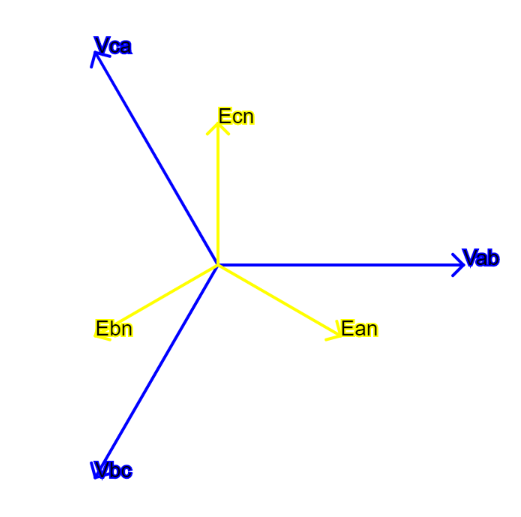
\includegraphics[width = 13cm]{fasores/fasores_de_tensao.png}
				\caption{Representação gráfica dos fasores }
			\end{figure}
			Determinando a corrente $I_{ac}$
			\[ \begin{split}
				&- E_{an} + I_{ac}X_c + I_{ac}R + E_{cn} = 0 \\
				&I_{ac} = \frac{-E_{ca}}{R+X_c}\\
				&I_{ac} = \frac{-100\measuredangle{ 120^\circ} }{50+\frac{1}{377\cdot 45.9E-6j}} \\
				&I_{ac} = 1.309 \measuredangle{-10.87^\circ} \text{ [A]}
			\end{split}
			\]
			Determinando a Tensão $V_{nN}$
			\[ \begin{split}
				&V_{nN} = - I_{ac}R + E_{cn}  \\
				&V_{nN} = 78.677 \measuredangle{-144.76^\circ} \text{ [V]}
			\end{split}
			\]
			Determinando V$_{f'N}$
			\[\begin{bmatrix}
				E_{a'N} \\
				E_{b'N} \\
				E_{c'N} \\
			\end{bmatrix}
			=
			\begin{bmatrix}
				57.7\measuredangle{-30^\circ} \\
				57.7\measuredangle{-150^\circ} \\
				57.7\measuredangle{90^\circ} \\
			\end{bmatrix}
			-VnN \cdot \begin{bmatrix}
				1\\
				1\\
				1\\
			\end{bmatrix}
			\]
			\[\begin{bmatrix}
				E_{a'N} \\
				E_{b'N} \\
				E_{c'N} \\
			\end{bmatrix}
			=
			\begin{bmatrix}
				115.45\measuredangle{8.23^\circ} \\
				136.27\measuredangle{-144.98^\circ} \\
				65.433\measuredangle{169.13^\circ} \\
			\end{bmatrix}
			\]
			Assim obtemos os fasores
			\begin{figure}[H]
				\centering % para centralizarmos a figura
				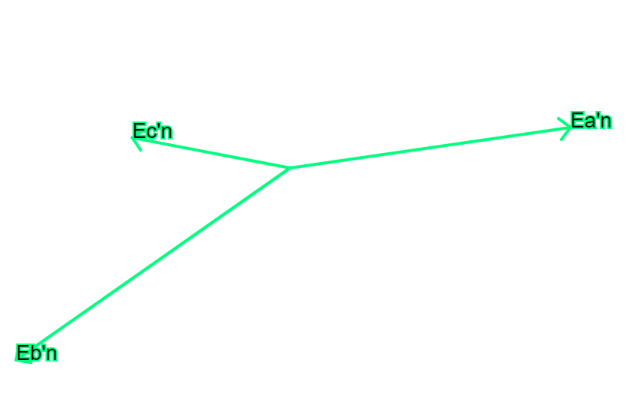
\includegraphics[width = 13cm]{fasores/seqabc.png}
				\caption{Representação gráfica dos fasores de tensão nos pontos a, b' e c' para sequência ABC}
			\end{figure}
			\newpage
			Fazendo o mesmo equacionamento para a sequencia CBA, obtém-se:
			\begin{figure}[H]
				\centering % para centralizarmos a figura
				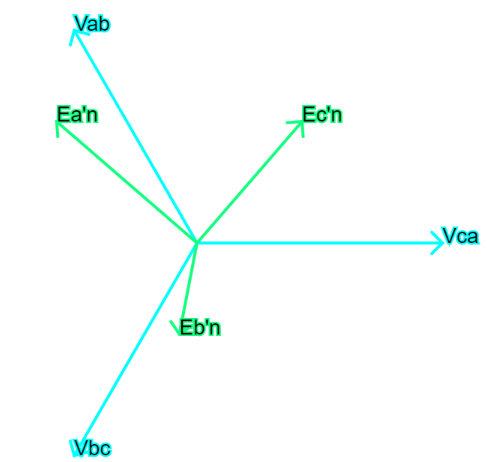
\includegraphics[width = 13cm]{fasores/cba.png}
				\caption{Representação gráfica dos fasores de tensão nos pontos a, b' e c' para sequência CBA}
			\end{figure}
			\newpage
			\justifying
			\subsection{Questões}
			\textbf{a) Na impossibilidade de ter voltímetros, amperímetros e sequencímetro, como você poderia
			encontrar a solução desse problema (abc ou cba)?
			}\\
			Utilizando lampadas incandescentes, em que a que estiver sujeita a maior tensão brilhará mais.
			
			\textbf{b) Aponte a importância de encontrar a correta sequência de fase em um circuito elétrico.}
			Determinar o sentido de giro de um motor.
			
			\newpage
			\section{Simulação}
		\justifying
		\newpage
		\section{Conclusão}
		\justifying
		\newpage
		\section*{Referencias}
		\justifying
		\noindent
		ALEXANDER, C.K.; SADIKU, M.N. Fundamentos de Circuitos Elétricos. 5ª ed.
		Porto Alegre: Mc Graw-Hill, 2015\\
		
		\noindent
		[1] - LIMA, H.S.; Desenhando Fasores https://xx220xx.github.io/FASORES/index.html acesso em 30/11/2019 \\
	\end{document}
